\begin{frame}
    \frametitle{Causalité ?}
\begin{itemize}
    \item Choisir un réseau avec des arêtes orientées pour représenter la causalité ?
    \pause 
\item Ex: Si F et G sont corrélés, l'un est-il la cause de l'autre ?

	 \pause 
	    \begin{center}
	     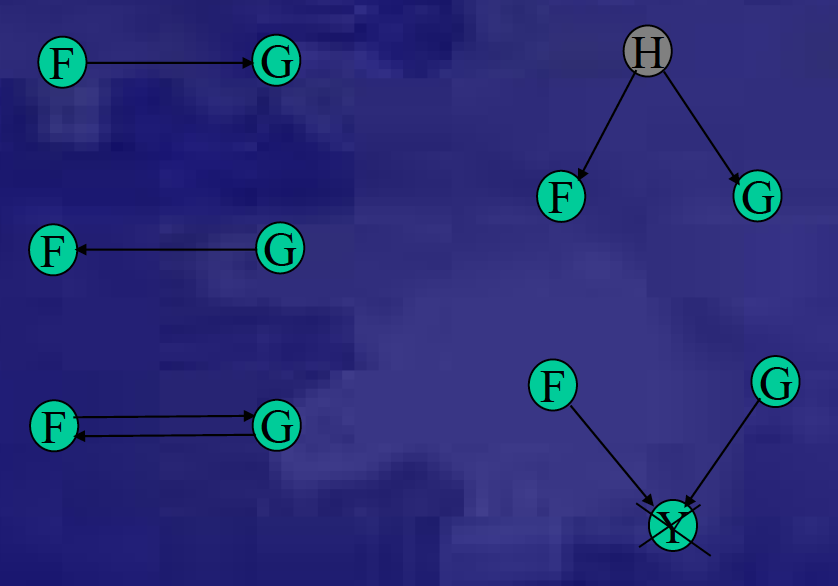
\includegraphics[width=6.5cm]{Figures/Causalité/F_et_G_corrélés.png}
	     	   \end{center}



\end{itemize}
\end{frame}

\begin{frame}
    \frametitle{Causalité ?}
\begin{itemize}
    \item Choisir un réseau avec des arêtes orientées pour représenter la causalité ?

\item Ex: Si F et G sont corrélés, l'un est-il la cause de l'autre ?

    
    \item Utiliser le formalisme des réseaux bayésiens ? 
    
    \begin{center}
    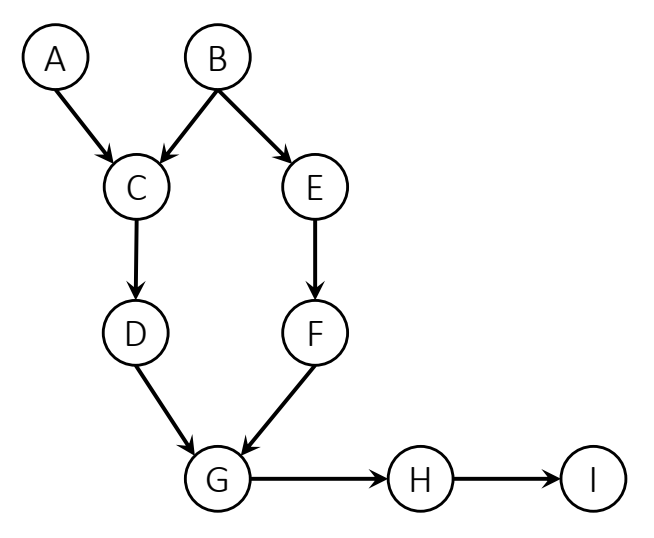
\includegraphics[width=5cm]{Figures/Causalité/BN.png}        
    \end{center}
    
\end{itemize}
\end{frame}




	 
 \begin{frame}
   \frametitle{Réseaux bayésiens }
   
   \begin{itemize}
       \item Les \textbf{modèles graphiques}
       \begin{itemize}
            \item Ce sont des \textbf{modèles probabilistes} pour la représentation des connaissances. 
            \item Ils reposent sur une description graphique des variables aléatoires.
            \item Objectif : représenter des distributions multi-dimensionnelles de grande taille (Utiliser les indépendances conditionnelles pour obtenir un réseau ‘sparse'). % en évitant l’explosion combinatoire.
       \end{itemize}
       
       \pause 
       
    \item 2 grandes classes de modèles très utilisées :
    \begin{itemize}
        \item Les \textbf{GGM} (cf. cours co-expression)
        \item Les \textbf{réseaux bayésiens}
        \begin{itemize}
            \item Représentation des dépendances par des arêtes orientées
            \item Utilisés pour modéliser les relations causales 
    \end{itemize}
    \end{itemize}
    
   \end{itemize}
   	\end{frame}




 \begin{frame}
   \frametitle{Mise en application des Réseaux bayésiens}
   
   Les réseaux bayésiens (RB) sont très utiles,\\
   \pause 
   
   \hspace{4cm} mais \textbf{attention au contexte} d'utilisation. 
   
  \pause
  
	 \begin{itemize}
 

\item \textbf{1ère limite} : Un RB est défini par un graphe orienté \textbf{acyclic} (ou DAG pour Directed Acyclic Graph)


Cex : Le motif ci-dessous ne peut pas être représenté par un RB.

    \begin{center}
    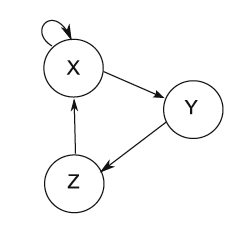
\includegraphics[width=4cm]{Figures/Causalité/XYZcycle.png}        
    \end{center}
    

    
\end{itemize}

	 \end{frame}
	 
    
     \begin{frame}
   \frametitle{Réseaux bayésiens : Définition}
   
	Soit $\mathcal{G}$ un graphe orienté \textbf{acyclic} (DAG)
	 \begin{itemize}
\item On appelle les \textbf{parents} d'un noeud $X_i$  l'ensemble des noeuds ayant une arête dirigée vers $X_i$. 
\pause 

\item Propriété/Définition : La distribution du vecteur aléatoire $X$ admet une représentation selon un \textbf{réseau bayésien} si et seulement si sa densité $f$ se factorise en un produit de densités conditionnelles de chaque variable $X_i$ sachant ses parents $pa(X_i,\mathcal{G})$ dans le graphe $\mathcal{G}$, 
$$ f(X) = \Pi_{i \in P} f(X_i\vert pa(X_i,\mathcal{G}) )$$

\pause 

$\rightsquigarrow$ Ceci permet de traduire des indépendances conditionnelles. 

%\item Exemple : DAG pour la densité qui se factorise comme suit
%$f_X(x) = f_{X_1}\ f_{X_2} \ f_{X_3} \ f_{X_4\vert X_1,X_2,X_3} \ f_{X_5\vert X_1,X_3}\ f_{X_6\vert X_4} \ f_{X_7\vert X_4,X_5}$ ?
\end{itemize}
	 \end{frame}




	
	 \begin{frame}{Exemple de GRN}
	 

	  \begin{center}
	     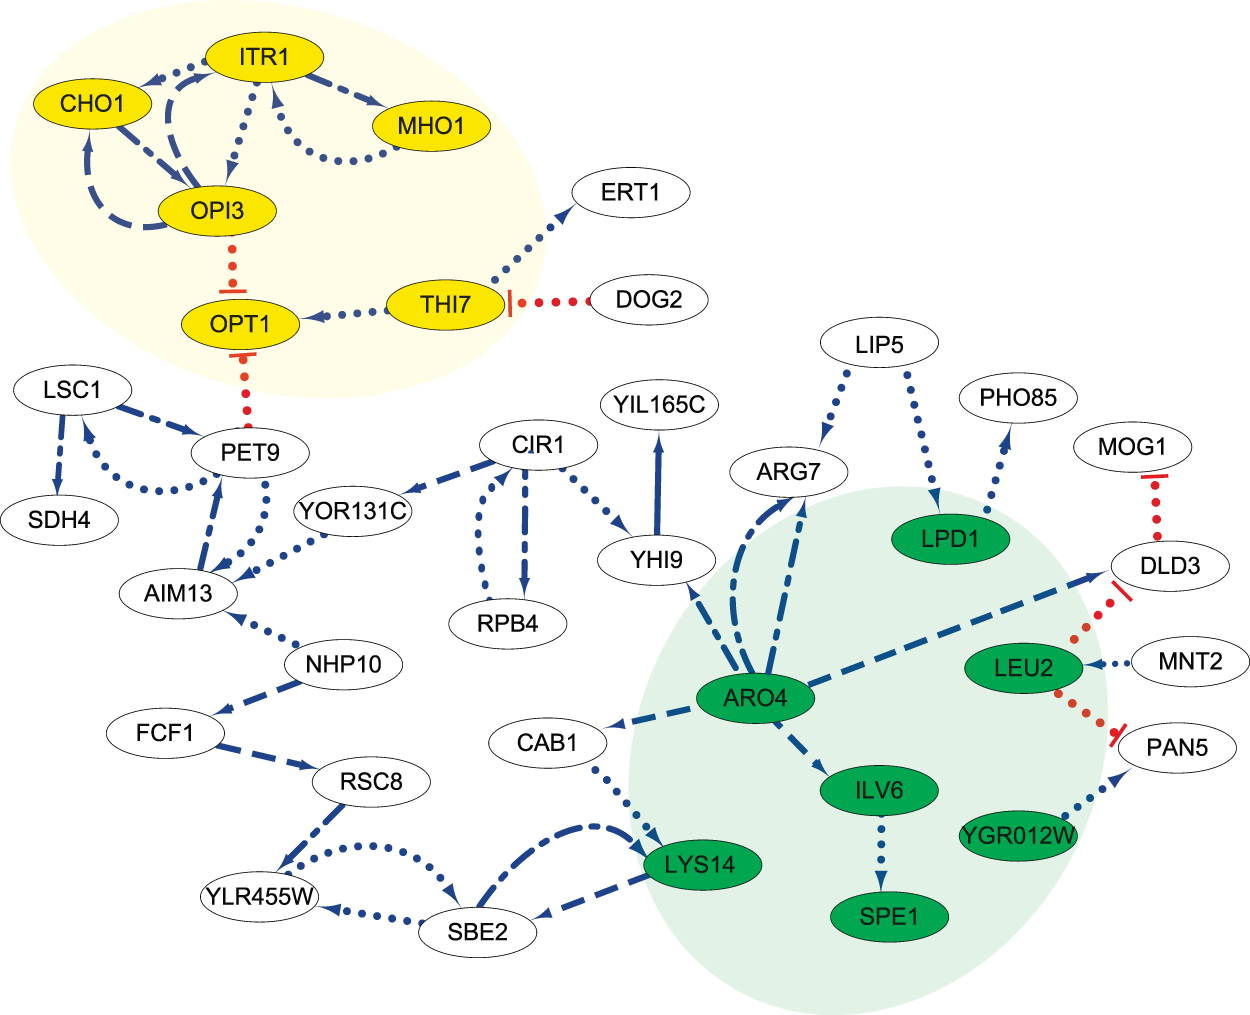
\includegraphics[width=6.5cm]{Figures/Causalité/gene_regulation_network.png}
	   \end{center}
	   
	   \vspace{-0.5cm}
	   
{\scriptsize \cite{ChenEtal2019}	   }

	   
\pause 


	  	  $\rightsquigarrow$ L'hypothèse de réseau sans cycle n'est pas naturelle pour un GRN. 
	  	  	 





	     
	     
	 \end{frame}
	 


\begin{frame}
   \frametitle{Mise en application des Réseaux bayésiens}
\vfill   
	 \begin{itemize}
\item \textbf{2ème limite} :  \textbf{Attention à l'interprétation} de l'orientation des arêtes.

\vfill
\pause

$\rightsquigarrow$ Des RBs différents peuvent représenter les mêmes indépendances conditionnelles. 

   \end{itemize}

\pause

   Ex : Le motif de régulation (A) peut être représenté par plusieurs DAG (B). 
   
	   \vspace{-0.2cm}

   	  \begin{center}
	    (A) 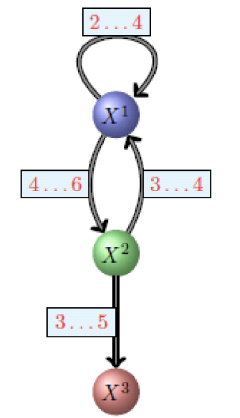
\includegraphics[width=2cm]{Figures/Causalité/reg_motif.png}\hspace{1cm}
	    (B) 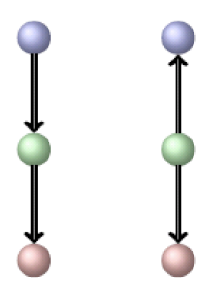
\includegraphics[width=3cm]{Figures/Causalité/DAG_motif.png}
	   \end{center}
	   
%   	\scriptsize \cite{LebreBMC10}   

	 \end{frame}


	\begin{frame}{Inférer un réseau causal}
	
	    Des méthodes ont cependant été développées pour \textbf{inférer un réseau causal}, notamment le \textbf{PC algorithm} qui permet d'inférer un réseau avec des arêtes orientées s'il est possible de le déduire des données, non orientées sinon.
	  
	   
    	   	\begin{center}
    	    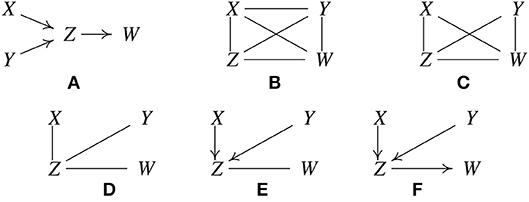
\includegraphics[scale = 0.5]{Figures/Causalité/PCalgo.jpeg}
    	\end{center}
    	
    	\pause 
    	
	    Pour aller plus loin : \textit{Review of Causal Discovery Methods Based on Graphical Models} \scriptsize \cite{GlymourZhangSpirtes2019}
	    
	    
	\end{frame}
		 


\begin{frame}
   \frametitle{Utiliser un \textbf{\textit{a priori} biologique}}
  \pause 
 
   
 \begin{itemize}
     \item[1)] \textbf{Le temps} : utiliser des données temporelles 
       \pause 
       
     $\rightsquigarrow$ Inférer les \textbf{dépendances temporelles} (réseau bayésien \textbf{dynamique}), \textit{i. e.} un réseau autorisant uniquement les arêtes entre un gène observé au  temps $t-1$ vers un gène observé au temps $t$.
     
        \pause 
        
   	  \begin{center}
	     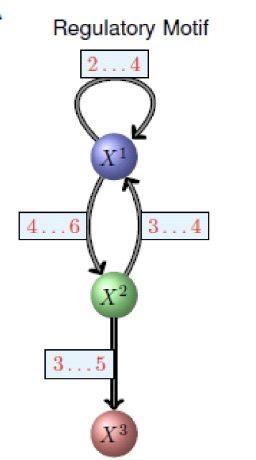
\includegraphics[width=2cm]{Figures/Causalité/motif.png}\hspace{1cm}
	     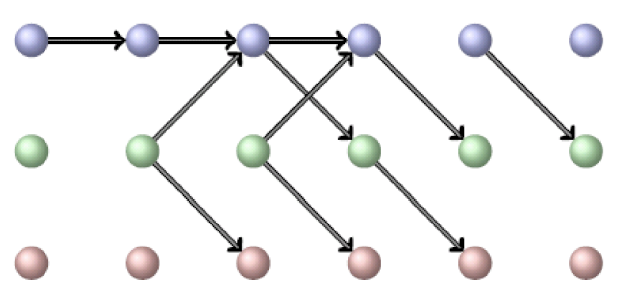
\includegraphics[width=7cm]{Figures/Causalité/TVDBN.png}
	   \end{center}
	   
	\scriptsize \cite{LebreBMC10}%,Dondelinger2013}   
	 %  Pour chaque gène observé au temps $t$, on recherche ses régulateurs parmi les gène observé au temps $t-1$,

 \end{itemize}  
\end{frame}
		 
		 
		 
\begin{frame}
   \frametitle{Utiliser un \textbf{\textit{a priori} biologique}}
   
 %  Une solution consiste à utiliser un \textit{a priori} biologique. 
   
 \begin{itemize}
     \item[2)] \textbf{La connaissance des facteurs de transcription (TF)} 
       \pause 
       
     \vfill
     
      $\rightsquigarrow$ Inférer les \textbf{dépendances transcriptionnelles}, \textit{i. e.} un réseau autorisant uniquement les arêtes orientée dans le sens :
     
\begin{center}
    TF $\rightarrow$  Gène cible
\end{center}

\pause

\vfill

Pour chaque gène cible, on recherche ses régulateurs parmi une liste de facteurs de transcription connus.
     
      
   	  \begin{center}
	 
	   \end{center}
 \end{itemize}  
 
 \end{frame}
		 
		 

	\begin{frame}
   \frametitle{Utiliser un \textbf{\textit{a priori} biologique}}
    	\vspace{-0.4cm}
    	\begin{center}
    	    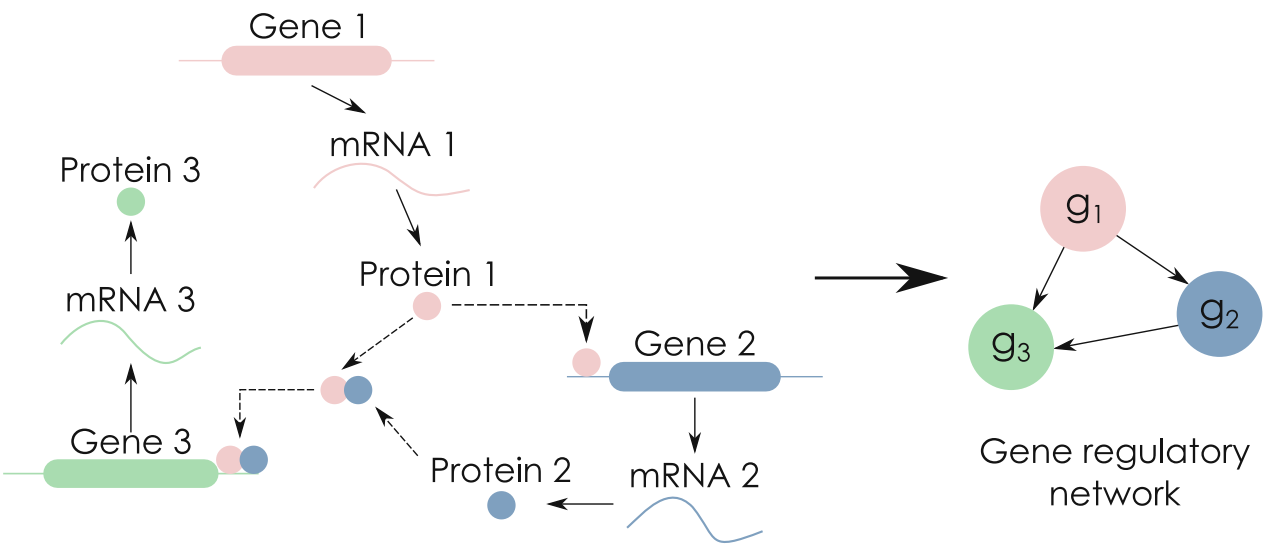
\includegraphics[scale = 0.33]{Figures/Intro/network.PNG}
    	\end{center}
    	\scriptsize \cite{sanguinetti2019gene}
    	
    	\onslide<2> 
    	
    	\begin{center}
\small    	
    	On considère que les niveaux d'expression des régulateurs $g_{1}, g_{2}$ vont permettre de prédire et d'expliquer les niveaux d'expression de $g_{3}$
    	\end{center}
	\end{frame}
	
	
	
		 
		 
\begin{frame}
   \frametitle{Se ramener à un problème de régression}
   Dans les deux cas, utiliser un \textit{a priori} biologique permet de se ramener à un problème de \textbf{régression}. 
   
   \vfill
   
   \pause 
   Il s'agit d'expliquer le niveau d'expression de chaque gène cible à partir : 
   \pause
   
   Cas 1 : des niveaux d'expressions des gènes observés au temps précédent
      \pause
      
Cas 2 : des niveaux d'expression des gènes connus comme facteurs de transcription

  
\end{frame}

	
